\section{Training}

An additional preprocessor was used to resample the fundamental frequency and loudness, taking into account the sample rate, frame rate, and the number of timesteps hyperparameters. The number of timesteps was set at 1000 per 4-second clip, giving a spectral resolution of 4ms per timestep. This timestep amount was deemed the best compromise between computational efficiency and accuracy.

The standard DDSP encoder-decoder setup was used except with the additional MFCC layer in the decoder as described previously in \nameref{sec:singing_voice_synthesis}.

The model settings were kept the same as in \nameref{sec:singing_voice_synthesis} as they had already validated their hyperparameter selection. Their hyperparameter selection included the use of 100 sinusoidal harmonic components and 60 filter banks; this was done to limit model size to ensure it fitted on one GPU.

Each model was trained for 200,000 epochs; the training time was approximately 2.9 epochs per second or 5.2 epochs per second, depending on the GPU. Total training time was approximately 20 hours per model.

\begin{figure}[H]
    \centering
    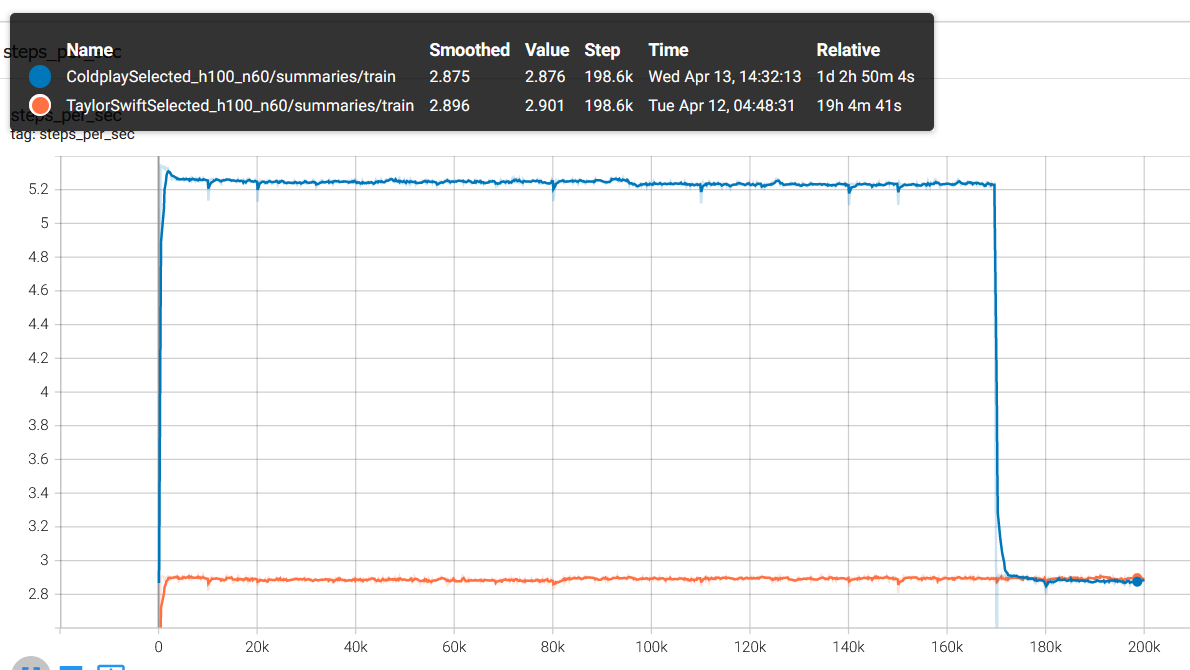
\includegraphics[width=0.6\textwidth]{research/training/StepsPerSecond.png}
    \caption{Training steps per second, on best hardware available in Google Colab sufficient training to 200,000 epochs could be achieved in approximately 11 hours (assuming 5 epochs per second).}
\end{figure}

\begin{figure}[H]
    \centering
    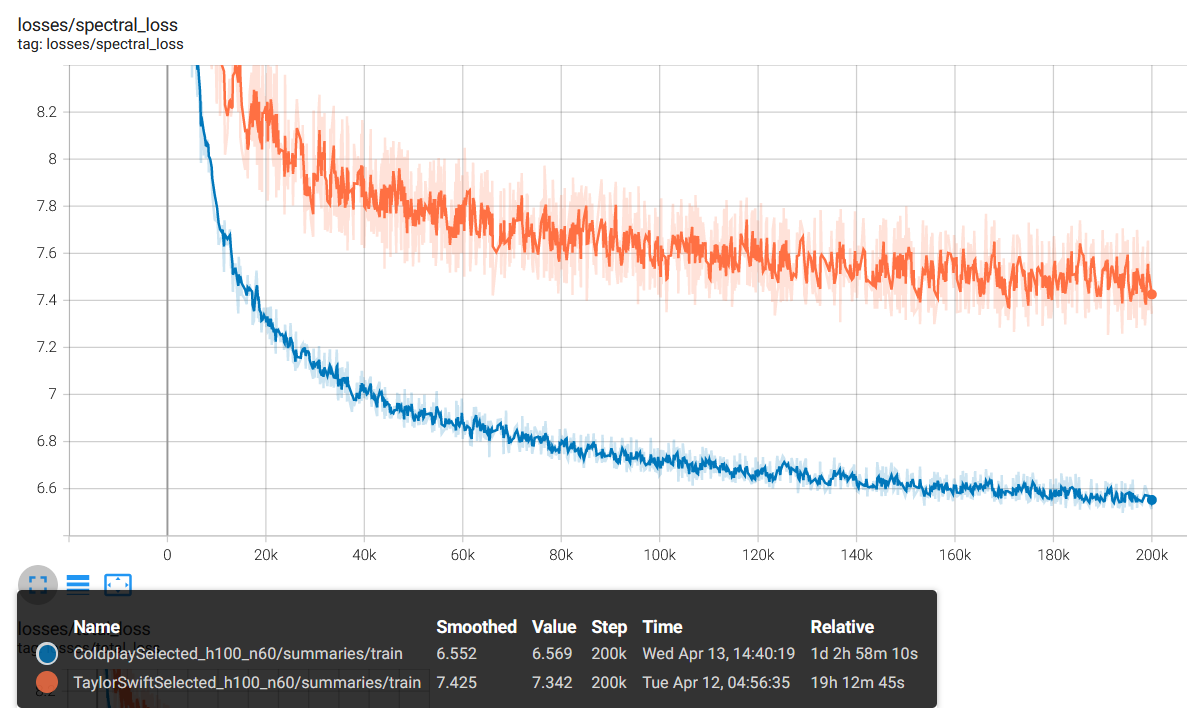
\includegraphics[width=0.8\textwidth]{research/training/TrainingSpectralLosses.png}
    \caption{Training Spectral Losses: Losses over the 200,000 epochs of training both models, using the spectral loss function defined in \nameref{sec:loss_measure}}
    \label{fig:training_spectral_losses}
\end{figure}

Figure \ref{fig:training_spectral_losses} shows the Coldplay losses being less than the Taylor Swift losses. The Coldplay Dataset has more pure silence frames, meaning that the Coldplay model fitted the silence frames more accurately. Furthermore, the Coldplay dataset was smaller than the Taylor Swift one.
